\subsection{Restos}

\odnote{Rodrigo: Mira si merece la pena integrar este texto en alg�n lado. No fuerces.}

El estudio etnogr�fico devel� varias situaciones problem�ticas en torno a la experimentaci�n en SE, particularmente en lo referente a la comunicaci�n debida a la diversidad terminol�gica y operativa existente en el grupo de investigaci�n estudiado. El survey abord� m�s expl�citamente la problem�tica en torno a la experimentaci�n en la comunicad de ESE. Encontramos que m�s de un 60\% de los investigadores encuestados consideran que la experimentaci�n en SE es compleja debido a distintos factores (ver Fig. \ref{fig-Factors-Influencing-Complexity-ESE}). Por ejemplo, un 33.33\% considera que la complejidad de la experimentaci�n se debe a que el {\color{green}(SC9)} \ul{low sample size results in weak arguments which avoid addressing the industrial problems}; mientras que un 11\% cree que {\color{green}(SC10)} \ul{the abundant range of statistical tests options and poor knowledge about it results in an erroneous statistical study}.

\begin{figure*}[htbp!]
	\centering
	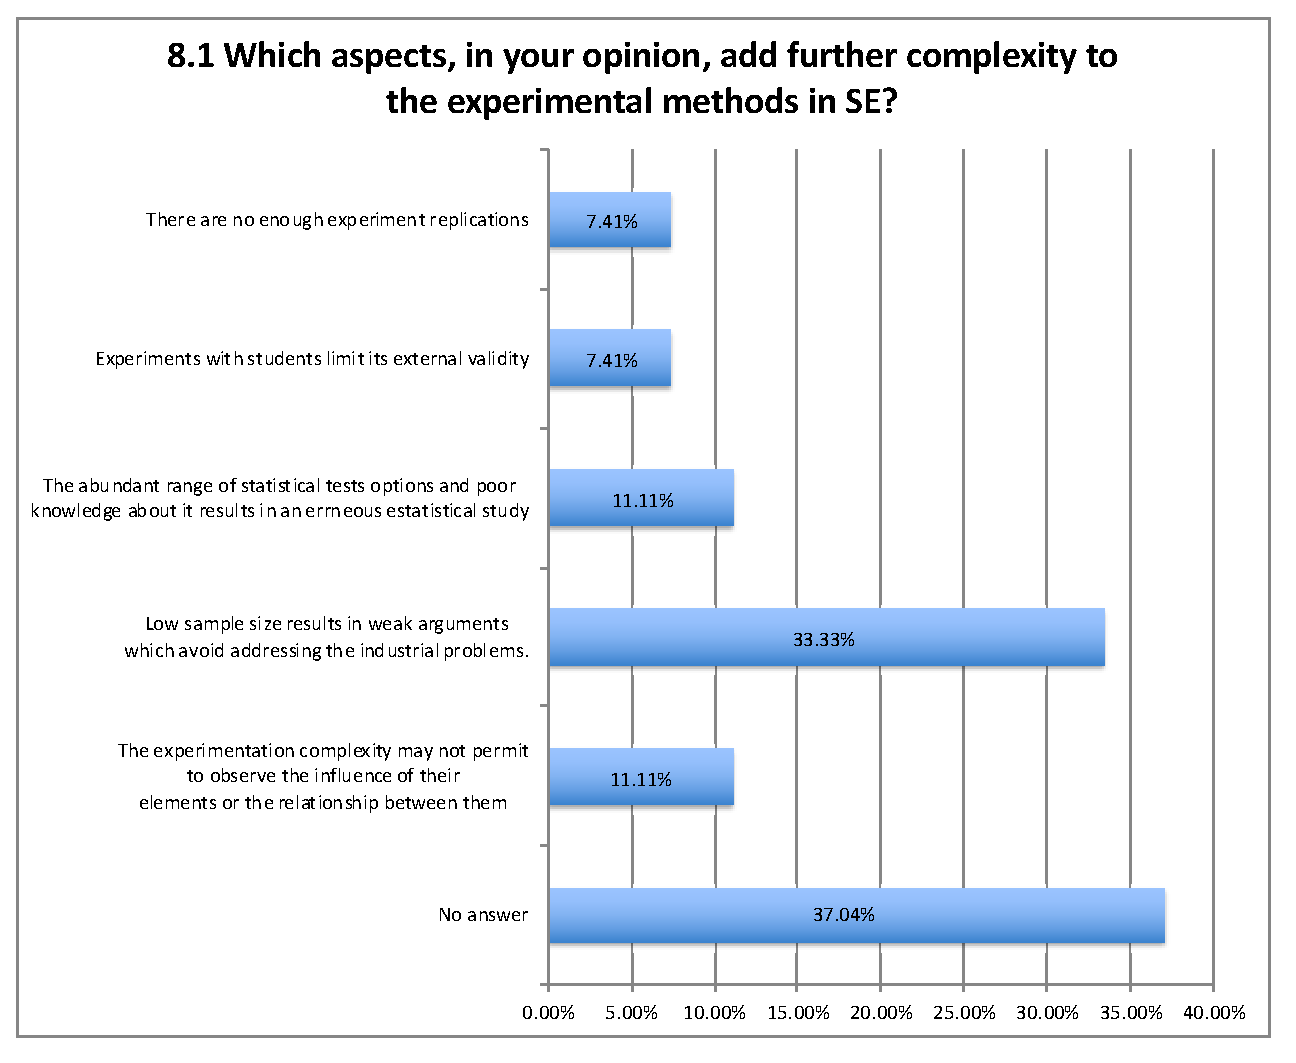
\includegraphics[width=12cm]{Images/Factors-Influencing-Complexity-ESE}
	\caption{Factors influencing the complexity of experimentation in SE}
	\label{fig-Factors-Influencing-Complexity-ESE}
\end{figure*}

As� mismo, un 11\% de los investigadores piensan que {\color{green}(SC11)} \ul{the experimentation complexity may not permit to observe the influence of their elements or the relationship between them}; mientras que otros investigadores son m�s espec�ficos y le atribuyen la complejidad de la experimentaci�n a que {\color{green}(SC12)} \ul{there are no enough experiment replications} (7.41\%) y a que los {\color{green}(SC13)} \ul{experiments with students limit its external validity} (7.41\%).

Por otra parte, otro problema remarcado en este estudio es el referido a la dificultad en la gesti�n de los datos. Un 14.81\% considera que {\color{green}(SC14)} \ul{el manejo y el an�lisis de los datos experimentales son complejos, lo que podr�a deberse en parte a las distintas maneras que tienen los investigadores para gestionarlos}: Un 66.67\% afirma que utilizan hojas de calculo, un 25\% repositorios de datos relacionales y un 44\% formatos propietarios. Por otra parte, un 7.41\% de los encuestados hace �nfasis en la limitada compartici�n de datos que existe, lo que es corroborado por mas de un 10\% de investigadores que consideran que {\color{green}(SC15)} \ul{la agregaci�n de datos entre replicaciones es compleja, quiz� en parte porque no existe un soporte adecuado para las replicaciones y la existencia del conocimiento t�cito}.

\begin{tcolorbox}

los aspectos que consideramos como problem�ticos en torno a la SE experimentation fueron corroborados en gran medida por los encuestados, e incluso se obtuvieron importantes recomendaciones a ser consideradas (ver Fig. \ref{fig-recommendations-improve-SE-experimentation}):

\begin{itemize}
  \item To have a common empirical source of knowledge
  \item To use simple guidelines to report findings
  \item To formalize the process
  \item To formalize the terminology
  \item To apply statistical test depending on experiment design
  \item To have a set of selected experimental subjects
  \item To receive quality formal courses
\end{itemize}

\end{tcolorbox}

\begin{figure*}[htbp!]
	\centering
	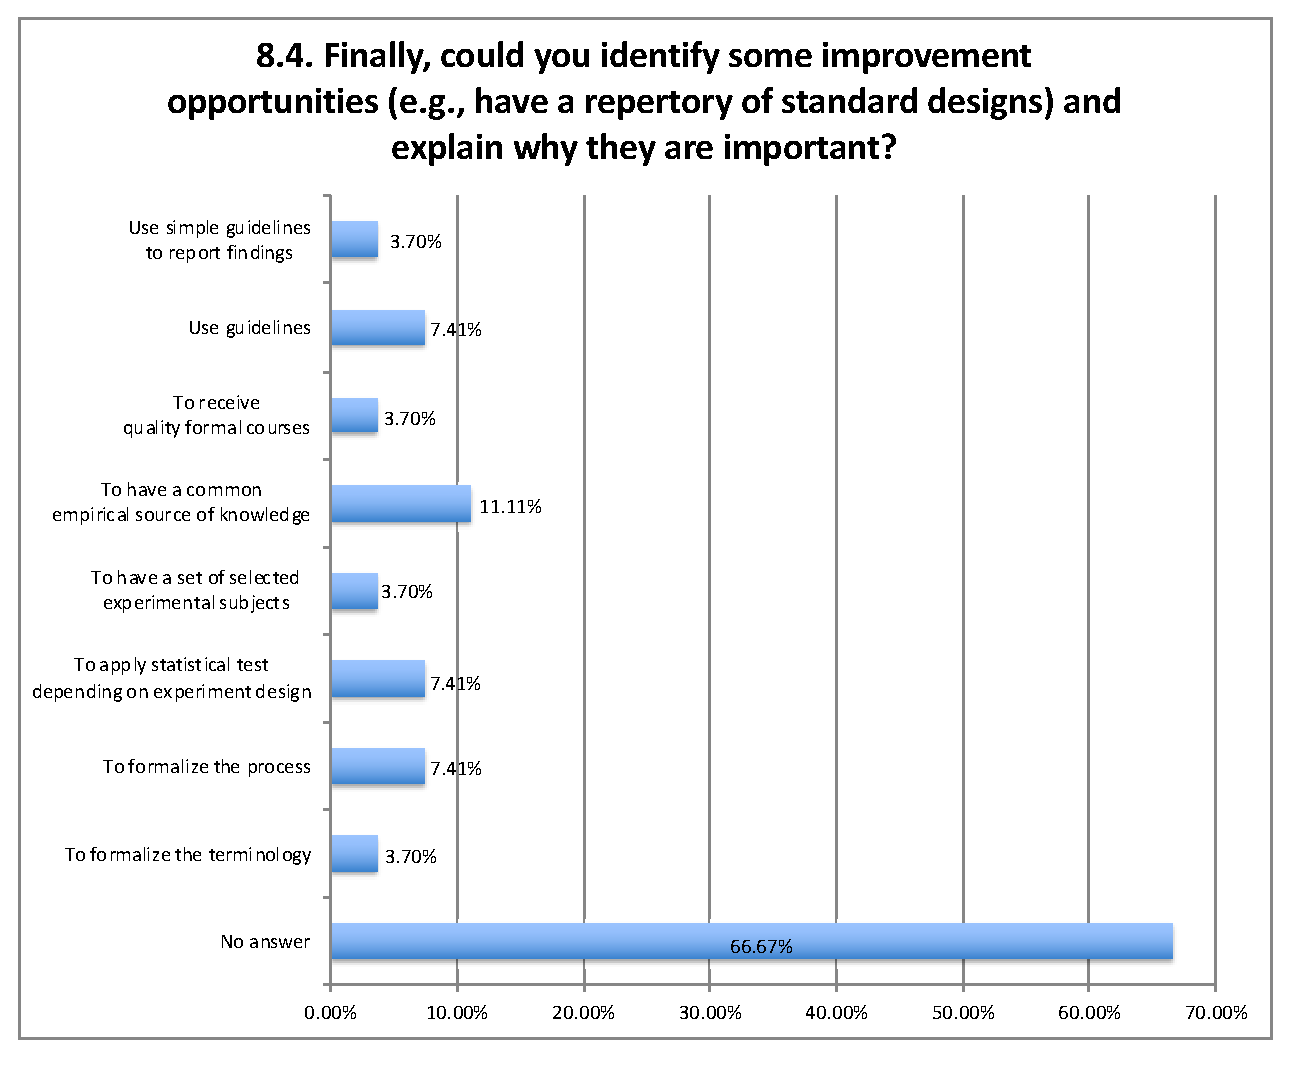
\includegraphics[width=12cm]{Images/Recommendations-Improve-SE-Experimentation}
	\caption{Recommendations to Improve the Experimentation in SE}
	\label{fig-recommendations-improve-SE-experimentation}
\end{figure*}